\documentclass{article}

\usepackage{amsmath, amsthm, amssymb}
\usepackage{geometry}
\geometry{margin = 3.0 cm}

\usepackage{enumerate}
\usepackage{url}

\usepackage{tikz}
\newcommand*\circled[1]{\tikz[baseline=(char.base)]{
            \node[shape=circle,draw,inner sep=2pt, color=red] (char) {#1};}}

\newcommand*\circledt[1]{\tikz[baseline=(char.base)]{
            \node[shape=circle,draw,inner sep=2pt, color=blue] (char) {#1};}}


\usepackage{algorithm}
\usepackage{caption}
\usepackage{algpseudocode}
\algblockdefx[NAME]{Input}{EndInput}
    [1][]{\textbf{Input:} #1}
    {}

\algblockdefx[NAME]{Output}{EndOutput}
    [1][]{\textbf{Output:} #1}
    {}

\newcommand{\myalg}[2]{\begin{figure}[H]
    { \renewcommand{\figurename}{Algorithm}
\begin{center}
\begin{minipage}{0.6\textwidth}
\hrulefill
\begin{algorithmic}[1]
    #1
\end{algorithmic}
\hrulefill
\end{minipage}
\end{center}
\caption{#2}
}
\end{figure}}

\renewcommand{\l}{\lambda}
\renewcommand{\L}{\Lambda}
\renewcommand{\mod}{~\mathrm{mod}~}
\renewcommand{\div}{~\mathrm{div}~}

\renewcommand{\vec}[1]{\mathbf{#1}}

\renewcommand{\(}{\left(}
\renewcommand{\)}{\right)}

\newcommand{\dist}{\text{dist}}

\newcommand{\mat}[1]{\begin{pmatrix} #1 \end{pmatrix}}
\newcommand{\room}{\hspace{0.5cm}}
\newcommand{\hl}[1]{\textbf{#1}}
\newcommand{\ceil}[1]{\lceil #1 \rceil}
\newcommand{\floor}[1]{\lfloor #1 \rfloor}

%\newcommand{\tm}{\textsuperscript{\texttrademark}}
\def\tm{$^{\hbox{\tiny TM}}$~}

\newtheorem{lem}{Lemma}

\usepackage{tikz} \usetikzlibrary{shapes}
\usetikzlibrary{arrows}

\tikzset{node distance=3cm, auto}

\title{Implementation of the BSP model for the Epiphany\tm architecture}
\author{Jan-Willem Buurlage \ Abe Wits \\ \normalsize{Utrecht University, The Netherlands}}

\begin{document}

\maketitle

\abstract{In this report we introduce the \texttt{epiphany-bsp} library, an implementation of the BSP model on the Epiphany\tm architecture. After introducing this architecture, we give some technical details of current hardware that ship with an Epiphany\tm chip. Next we describe the BSP library that we developed.}

\tableofcontents

\newpage

\setlength{\parskip}{0.2 cm}
\setlength{\parindent}{0.0 cm}

\section{Introduction}

The Epiphany\tm architecture is a multicore microprocessor architecture that was developed by Adapteva\footnote{\url{http://www.adapteva.com}}. The Epiphany\tm architecture is implemented on chips that are inteded as a coprocessor to ARM/Intel CPUs. Every core has access to local, and shared memory. Besides the Epiphany\tm technology Adapteva has developed the Parallella board\footnote{\url{http://www.parallella.org}}, which is a computer with the size of a credit card that is based on this multicore coprocessor technology.

\subsection{The Epiphany\tm architecture}

The Epiphany architecture consists of 1 to 4096 Reduced Instruction Set Computer (RISC) cores, with local memory. These cores are part of a multicore framework. Besides this there is a Network-On-Chip (NOC) present, designed for real time applications. \ldots

\subsubsection{Memory model}

\subsection{Parallella Board}

Toy model, new architecture

\subsubsection{Memory}

\section{BSP on Epiphany}

\subsection{Design choices}

\subsection{Primitives}

\section{Optimizations}

\section{Examples}

\section{Performance Measurements}

\subsection{BSP parameters / benchmark}

\subsection{GFlops/Watt etc.}
The 64-core Epiphany-IV chip is (one of the) most efficient processors measured in single precision GFLOPs/W. However, the total amount of GFLOPs is relatively low. Adapteva (the developing company) claims that the techniques used are scalable, and more powerfull chips with comparable power consumption are developed. If Adapteva can deliver on its promices, Epiphany chips could play a role in future super computers.

16 core Parallela has roughly 5.0 GFLOPs/W, 64 core Epiphany-IV 50 GFLOPs/W. (wiki)
16 core Parallela costs about 94 euros
\#1 of Green500 computers is at about 3.0 GFLOPs/W (2013)
Epiphany-IV is the most efficient according to this source:
http://streamcomputing.eu/blog/2012-08-27/processors-that-can-do-20-gflops-watt/

\section{Further Work}

\subsection{Clusters etc.}

\section{A1: The Epiphany chip}
The Epiphany architecture consists of a grid of processors.
\subsection{The Epiphany System Programming Model}
The grid of processors is defined as a rectangle in the Epiphany Space. In this space we can define rectangular \textit{Workgroups} using two points; a Workgroup Origin and a Workgroup Size. We can refer to processors (we call the active processor the \textit{eCore}) in this Workspace using relative coordinates; (0,0) refers to the Workgroup Origin.
\begin{centering}
\begin{figure}
\centering
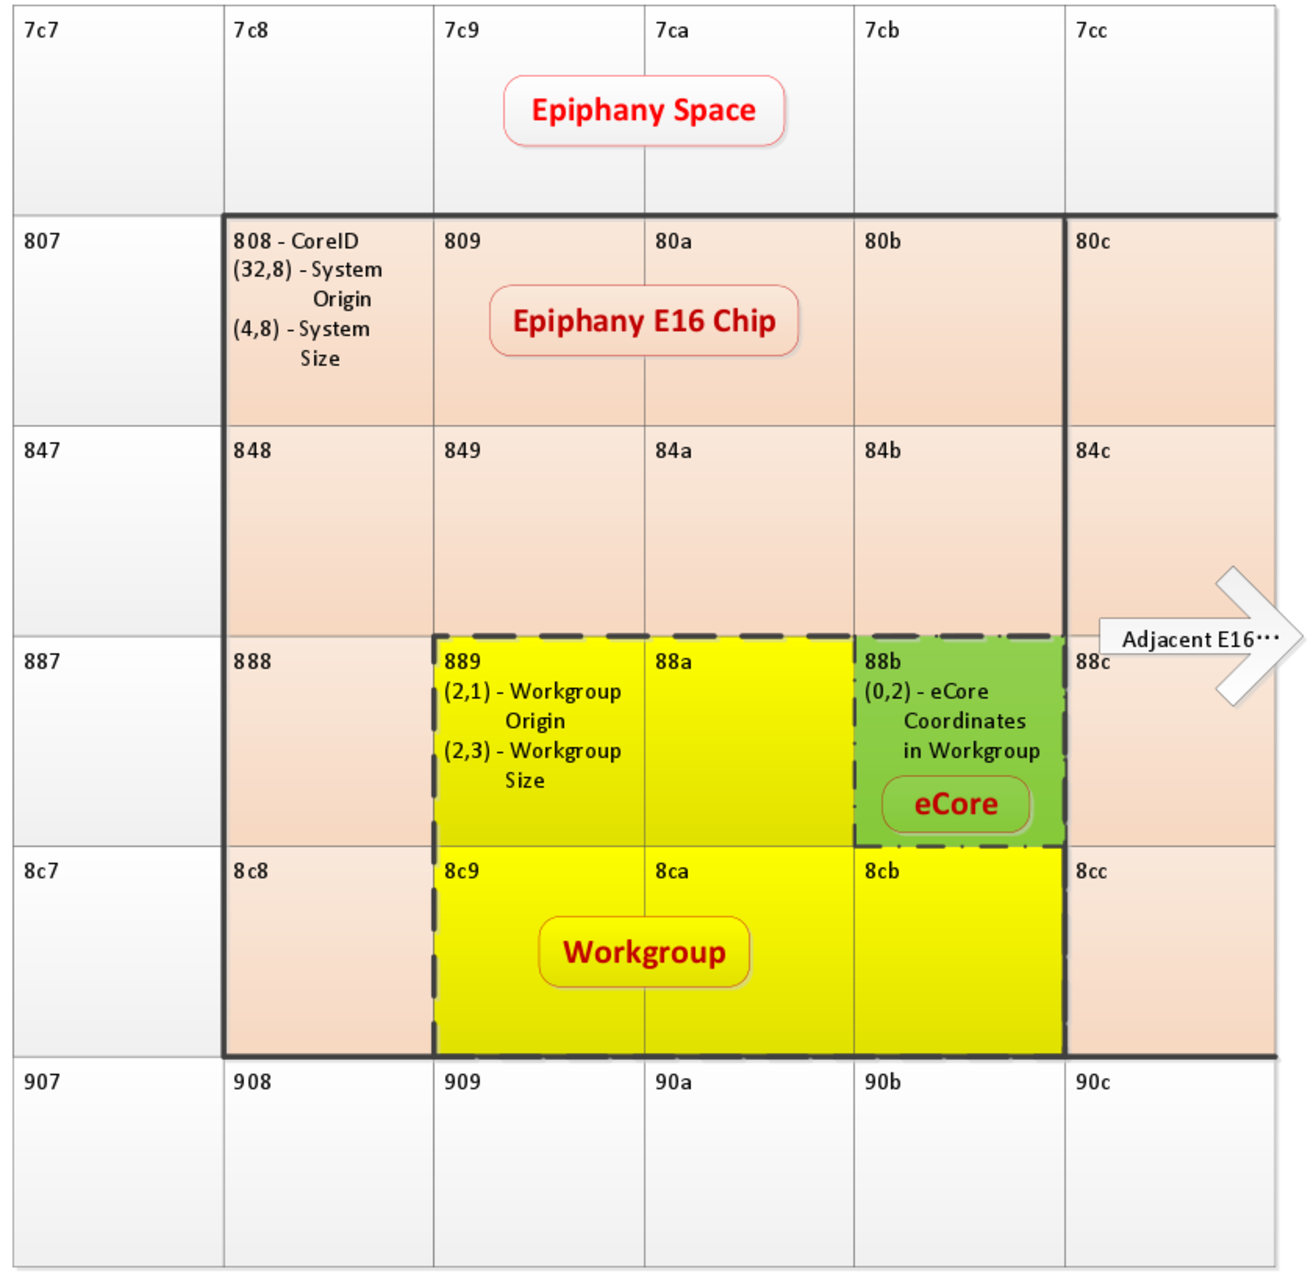
\includegraphics[scale=0.5]{EpiphanySpace.pdf}
\caption{The Epiphany Platform, Workgroup an eCore coordinates. Source: Adapteva Inc. Epiphany SDK Reference}
\end{figure}
\end{centering}
\section{A2: Installing \texttt{epiphany-bsp}}

\subsection{Prerequisites}

We use the 2014-08 release of the Epiphany SDK (eSDK), notes on installing this can be found here: \url{https://github.com/adapteva/epiphany-sdk/wiki/Notes-on-the-2014.08-release}.

First of all, on Ubuntu Linux we have to install the following packages:
\begin{align*} 
    &\texttt{sudo apt-get install u-boot-tools gcc-4.8-arm-linux-gnueabihf g++-4.8-arm-linux-gnueabihf} \\
    &\texttt{\hspace{1 cm}> bison flex libgmp-dev libncurses-dev libmpc-dev libmpfr-dev texinfo xzip lzip}
\end{align*}
Next, after cloning the \verb+epiphany-sdk+ repoistory we checkout the \texttt{2014.08.rc} branch.

When downloading the toolchain, we \verb+--clone+ to make sure we obtain the latest sources (allegedly else it will download outdated ones). Else the toolchain will then build for the build machine, but it might complain along the lines of \texttt{archive has no index}. We run \texttt{arm-linux-gnueabihf-ranlib} for all these archives to try and fix this, but to no avail...


\subsection{Obtaining the source}

\subsection{Example usage}

\section{References}

\begin{enumerate}
    \item \url{http://www.adapteva.com/white-papers/building-the-worlds-first-parallella-beowulf-cluster/}
    \item \url{http://www.adapteva.com/}
    \item \url{http://www.parallella.org}
    \item \url{MulticoreBSP}
    \item \url{BSPlib}
\end{enumerate}

\section{TODO}

Make epiphany-examples shared, symbolic link home folders abe jw

\end{document}
